\documentclass{article}

% Language setting
% Replace `english' with e.g. `spanish' to change the document language
\usepackage[english]{babel}

% Set page size and margins
% Replace `letterpaper' with `a4paper' for UK/EU standard size
\usepackage[letterpaper,top=2cm,bottom=2cm,left=3cm,right=3cm,marginparwidth=1.75cm]{geometry}

% Useful packages
\usepackage{amsmath, amsfonts, amssymb}
\usepackage{graphicx}
\usepackage{todonotes}
\usepackage[dvipsnames]{xcolor}
\usepackage{tikz,tikz-cd}
\usepackage[colorlinks=true, allcolors=blue]{hyperref}

\newcommand{\Z}{\mathbb{Z}}
\newcommand{\DD}{\mathcal{D}}
\newcommand{\gr}{\mathsf{gr}}
\newcommand{\KK}{\mathbf{K}}
\newcommand{\G}{\mathsf{G}}
\newcommand{\id}{\mathrm{id}}
\newcommand{\uone}{U(1)}
\newcommand{\Q}{\mathbb{Q}}
\renewcommand{\sc}{\; ; \;}

\DeclareMathOperator{\Ext}{Ext}
\DeclareMathOperator{\Hom}{Hom}
\DeclareMathOperator{\Res}{Res}
\DeclareMathOperator{\Quo}{Quo}




\newcommand{\sdr}[5]{%
  \begin{tikzcd}[column sep=large, ampersand replacement=\&]
    {#1} \arrow[r, "#3", shift left=0.5ex,] \arrow[r, leftarrow, "#4", shift right=0.5ex, swap] \& 
    {#2} \arrow[loop right, distance=1em, in=15, out=-15, "#5",swap]
  \end{tikzcd}%
}

\newcommand{\mf}[4]{%
  \begin{tikzcd}[column sep=3.5cm, ampersand replacement=\&]
    {#1} \arrow[r, "#3", shift left=0.5ex, bend left=5,start anchor=east, end anchor=west] \arrow[r, leftarrow, "#4", shift right=0.5ex, bend right=5, swap, start anchor=east, end anchor=west] \& 
    {#2}
  \end{tikzcd}%
}

\newcommand{\mfshort}[4]{%
  \begin{tikzcd}[ampersand replacement=\&]
    {#1} \arrow[r, "#3", bend left=5,start anchor=east, end anchor=west, shift left=2pt]  \& 
    {#2} \arrow[l,"#4", bend left=5, start anchor=west, end anchor=east, shift left=2pt]
  \end{tikzcd}%
}



\newcommand{\rarmf}[1]{%
 \arrow[r, "#1", shift left=0.5ex, bend left=10]
}

\newcommand{\larmf}[1]{%
 \arrow[r, leftarrow, "#1", shift right=0.5ex, bend right=10, swap] 
}


 \newcommand{\ThickEdgeStandard}{
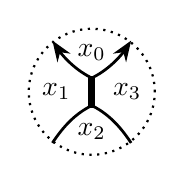
\begin{tikzpicture}[thick,baseline=(current bounding box.center)]

% Dotted circle
\draw[dotted,thick] (0,0) circle (0.8cm);

% Central thick edge
\draw[line width=2.5pt] (0,0.2) -- (0,-0.2);

% Four thinner connecting edges
\draw[line width=1pt, -Stealth]
  (-0.01,0.18) .. controls (-0.25,0.3) and (-0.4,0.5) .. (-0.5,0.65); % upper left
\draw[line width=1pt, -Stealth]
  (0.01,0.18) .. controls (0.25,0.3) and (0.4,0.5) .. (0.5,0.65);   % upper right
\draw[line width=1pt]
   (-0.01,-0.18) .. controls (-0.25,-0.3) and (-0.4,-0.5) .. (-0.5,-0.65); % lower left
\draw[line width=1pt]
   (0.01,-0.18) .. controls (0.25,-0.3) and (0.4,-0.5) .. (0.5,-0.65);   % lower right

% Labels for regions
\node at (0,0.5) {$x_0$};
\node at (-0.45,0) {$x_1$};
\node at (0,-0.5) {$x_2$};
\node at (0.45,0) {$x_3$};

\end{tikzpicture}
}
\newcommand{\ThickEdge}[4]{
\begin{tikzpicture}[thick,baseline=(current bounding box.center)]

% Dotted circle
\draw[dotted,thick] (0,0) circle (0.8cm);

% Central thick edge
\draw[line width=2.5pt] (0,0.2) -- (0,-0.2);

% Four thinner connecting edges
\draw[line width=1pt, -Stealth]
  (-0.01,0.18) .. controls (-0.25,0.3) and (-0.4,0.5) .. (-0.5,0.65); % upper left
\draw[line width=1pt, -Stealth]
  (0.01,0.18) .. controls (0.25,0.3) and (0.4,0.5) .. (0.5,0.65);   % upper right
\draw[line width=1pt]
   (-0.01,-0.18) .. controls (-0.25,-0.3) and (-0.4,-0.5) .. (-0.5,-0.65); % lower left
\draw[line width=1pt]
   (0.01,-0.18) .. controls (0.25,-0.3) and (0.4,-0.5) .. (0.5,-0.65);   % lower right

% Labels for regions
\node at (0,0.5) {$#1$};
\node at (-0.45,0) {$#2$};
\node at (0,-0.5) {$#3$};
\node at (0.45,0) {$#4$};

\end{tikzpicture}
}

\newcommand{\ThinEdgeStandard}{
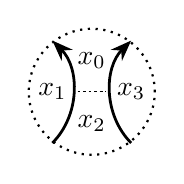
\begin{tikzpicture}[thick,baseline=(current bounding box.center)]

% Dotted circle
\draw[dotted,thick] (0,0) circle (0.8cm);

% Central dotted edge
\draw[dotted, dash pattern=on 1pt off 1pt, line width=0.5pt] (-0.18,0) -- (0.18,0);

% Four thinner connecting edges
\draw[line width=1pt, -Stealth]
  (-0.5,-0.65) .. controls (-0.15,-0.3) and (-0.15,0.3) .. (-0.5,0.65); % left
\draw[line width=1pt, -Stealth]
  (0.5,-0.65) .. controls (0.15,-0.3) and (0.15,0.3) .. (0.5,0.65);   %  right


% Labels for regions
\node at (0,0.4) {$x_0$};
\node at (-0.5,0) {$x_1$};
\node at (0,-0.4) {$x_2$};
\node at (0.5,0) {$x_3$};

\end{tikzpicture}
}
\newcommand{\ThinEdge}[4]{
\begin{tikzpicture}[thick,baseline=(current bounding box.center)]

% Dotted circle
\draw[dotted,thick] (0,0) circle (0.8cm);

% Central dotted edge
\draw[dotted, dash pattern=on 1pt off 1pt, line width=0.5pt] (-0.18,0) -- (0.18,0);

% Four thinner connecting edges
\draw[line width=1pt, -Stealth]
  (-0.5,-0.65) .. controls (-0.15,-0.3) and (-0.15,0.3) .. (-0.5,0.65); % left
\draw[line width=1pt, -Stealth]
  (0.5,-0.65) .. controls (0.15,-0.3) and (0.15,0.3) .. (0.5,0.65);   %  right


% Labels for regions
\node at (0,0.4) {$#1$};
\node at (-0.5,0) {$#2$};
\node at (0,-0.4) {$#3$};
\node at (0.5,0) {$#4$};

\end{tikzpicture}
}

\newcommand{\BigonStandard}[1]{
\begin{tikzpicture}[thick,baseline=(current bounding box.center)]

% Dotted circle
\draw[dotted,thick] (0,0) circle (1cm);

% Thick edges
\draw[line width=2.5pt] (0,0.25) -- (0,0.5);
\draw[line width=2.5pt] (0,-0.25) -- (0,-0.5);

% Four thinner connecting edges
\draw[line width=1pt, -Stealth]
  (-0.01,0.48) .. controls (-0.2, 0.55) and (-0.35,0.65)  .. (-0.5,0.87); % upper left
\draw[line width=1pt, -Stealth]
  (0.01,0.48) .. controls (0.2, 0.55) and (0.35,0.65)  .. (0.5,0.87);   % upper right
\draw[line width=1pt]
  (-0.01,-0.48) .. controls (-0.2, -0.55) and (-0.35,-0.65)  .. (-0.5,-0.87); % lower left
\draw[line width=1pt]
  (0.01,-0.48) .. controls (0.2, -0.55) and (0.35,-0.65)  .. (0.5,-0.87);   % lower right
\draw[line width=1pt]
  (0,0) circle (0.26cm);   % lower right

% Labels for regions
\node at (0,0) {$#1$};
\node at (0,0.75) {$x_0$};
\node at (-0.6,0) {$x_1$};
\node at (0,-0.75) {$x_2$};
\node at (0.6,0) {$x_3$};


\end{tikzpicture}
}
\newcommand{\Bigon}[5]{
\begin{tikzpicture}[thick,baseline=(current bounding box.center)]

% Dotted circle
\draw[dotted,thick] (0,0) circle (1cm);

% Thick edges
\draw[line width=2.5pt] (0,0.25) -- (0,0.5);
\draw[line width=2.5pt] (0,-0.25) -- (0,-0.5);

% Four thinner connecting edges
\draw[line width=1pt, -Stealth]
  (-0.01,0.48) .. controls (-0.2, 0.55) and (-0.35,0.65)  .. (-0.5,0.87); % upper left
\draw[line width=1pt, -Stealth]
  (0.01,0.48) .. controls (0.2, 0.55) and (0.35,0.65)  .. (0.5,0.87);   % upper right
\draw[line width=1pt]
  (-0.01,-0.48) .. controls (-0.2, -0.55) and (-0.35,-0.65)  .. (-0.5,-0.87); % lower left
\draw[line width=1pt]
  (0.01,-0.48) .. controls (0.2, -0.55) and (0.35,-0.65)  .. (0.5,-0.87);   % lower right
\draw[line width=1pt]
  (0,0) circle (0.26cm);   % middle

% Labels for regions
\node at (0,0) {$#1$};
\node at (0,0.75) {$#2$};
\node at (-0.6,0) {$#3$};
\node at (0,-0.75) {$#4$};
\node at (0.6,0) {$#5$};


\end{tikzpicture}
}

\newcommand{\ThinThickStandard}[1]{
\begin{tikzpicture}[thick,baseline=(current bounding box.center)]

% Dotted circle
\draw[dotted,thick] (0,0) circle (1cm);

% Thick and thin edge
\draw[dotted, dash pattern=on 1pt off 1pt, line width=0.5pt] (-0.2,0.36) -- (0.2,0.36);
\draw[line width=2.5pt] (0,-0.25) -- (0,-0.5);

% Four thinner connecting edges
\draw[line width=1pt, -Stealth]
  (-0.01,-0.27) .. controls (-0.7, -0.2) and (0.1,0.3)  .. (-0.5,0.87); % upper left
\draw[line width=1pt, -Stealth]
(0.01,-0.27) .. controls (0.7, -0.2) and (-0.1,0.3)  .. (0.5,0.87);   % upper right
\draw[line width=1pt]
  (-0.01,-0.48) .. controls (-0.2, -0.55) and (-0.35,-0.65)  .. (-0.5,-0.87); % lower left
\draw[line width=1pt]
  (0.01,-0.48) .. controls (0.2, -0.55) and (0.35,-0.65)  .. (0.5,-0.87);   % lower right


% Labels for regions
\node at (0,0) {$#1$};
\node at (0,0.65) {$x_0$};
\node at (-0.65,0) {$x_1$};
\node at (0,-0.75) {$x_2$};
\node at (0.65,0) {$x_3$};


\end{tikzpicture}
}
\newcommand{\ThinThick}[5]{
\begin{tikzpicture}[thick,baseline=(current bounding box.center)]

% Dotted circle
\draw[dotted,thick] (0,0) circle (1cm);

% Thick and thin edge
\draw[dotted, dash pattern=on 1pt off 1pt, line width=0.5pt] (-0.2,0.36) -- (0.2,0.36);
\draw[line width=2.5pt] (0,-0.25) -- (0,-0.5);

% Four thinner connecting edges
\draw[line width=1pt, -Stealth]
  (-0.01,-0.27) .. controls (-0.7, -0.2) and (0.1,0.3)  .. (-0.5,0.87); % upper left
\draw[line width=1pt, -Stealth]
(0.01,-0.27) .. controls (0.7, -0.2) and (-0.1,0.3)  .. (0.5,0.87);   % upper right
\draw[line width=1pt]
  (-0.01,-0.48) .. controls (-0.2, -0.55) and (-0.35,-0.65)  .. (-0.5,-0.87); % lower left
\draw[line width=1pt]
  (0.01,-0.48) .. controls (0.2, -0.55) and (0.35,-0.65)  .. (0.5,-0.87);   % lower right


% Labels for regions
\node at (0,0) {$#1$};
\node at (0,0.65) {$#2$};
\node at (-0.65,0) {$#3$};
\node at (0,-0.75) {$#4$};
\node at (0.65,0) {$#5$};


\end{tikzpicture}
}



\newcommand{\ThickThinStandard}[1]{
\begin{tikzpicture}[thick,baseline=(current bounding box.center)]

% Dotted circle
\draw[dotted,thick] (0,0) circle (1cm);

% Thick and thin edge (flipped vertically)
\draw[dotted, dash pattern=on 1pt off 1pt, line width=0.5pt] (-0.25,-0.38) -- (0.25,-0.38);
\draw[line width=2.5pt] (0,0.25) -- (0,0.5);

% Four thinner connecting edges (flipped vertically)
\draw[line width=1pt]
  (-0.01,0.27) .. controls (-0.7,0.2) and (0.1,-0.3) .. (-0.5,-0.87); % lower left 
\draw[line width=1pt]
  (0.01,0.27) .. controls (0.7,0.2) and (-0.1,-0.3) .. (0.5,-0.87);  % lower right 
\draw[line width=1pt, -Stealth]
  (-0.01,0.48) .. controls (-0.2,0.55) and (-0.35,0.65) .. (-0.5,0.87); % upper left
\draw[line width=1pt, -Stealth]
  (0.01,0.48) .. controls (0.2,0.55) and (0.35,0.65) .. (0.5,0.87);    % upper right

% Labels for regions
\node at (0,0) {$#1$};
\node at (0,0.75) {$x_0$};
\node at (-0.65,0) {$x_1$};
\node at (0,-0.65) {$x_2$};
\node at (0.65,0) {$x_3$};

\end{tikzpicture}
}
\newcommand{\ThickThin}[5]{
\begin{tikzpicture}[thick,baseline=(current bounding box.center)]

% Dotted circle
\draw[dotted,thick] (0,0) circle (1cm);

% Thick and thin edge (flipped vertically)
\draw[dotted, dash pattern=on 1pt off 1pt, line width=0.5pt] (-0.25,-0.38) -- (0.25,-0.38);
\draw[line width=2.5pt] (0,0.25) -- (0,0.5);

% Four thinner connecting edges (flipped vertically)
\draw[line width=1pt]
  (-0.01,0.27) .. controls (-0.7,0.2) and (0.1,-0.3) .. (-0.5,-0.87); % lower left 
\draw[line width=1pt]
  (0.01,0.27) .. controls (0.7,0.2) and (-0.1,-0.3) .. (0.5,-0.87);  % lower right
\draw[line width=1pt, -Stealth]
  (-0.01,0.48) .. controls (-0.2,0.55) and (-0.35,0.65) .. (-0.5,0.87); % upper left
\draw[line width=1pt, -Stealth]
  (0.01,0.48) .. controls (0.2,0.55) and (0.35,0.65) .. (0.5,0.87);    % upper right


% Labels for regions
\node at (0,0) {$#1$};
\node at (0,0.75) {$#2$};
\node at (-0.65,0) {$#3$};
\node at (0,-0.65) {$#4$};
\node at (0.65,0) {$#5$};

\end{tikzpicture}
}

\newcommand{\SquareStandard}[1]{
\begin{tikzpicture}[thick,baseline=(current bounding box.center)]

% Dotted circle
\draw[dotted,thick] (0,0) circle (1cm);

% Thick edges
\draw[line width=2.5pt] (-0.4,-0.2) -- (-0.4,0.2);
\draw[line width=2.5pt] (0.4,-0.2) -- (0.4,0.2);

% Thinner connecting edges
\draw[line width=1pt, -Stealth]
  (-0.42,0.18) .. controls (-0.5, 0.3) and (-0.55,0.45)  .. (-0.6,0.8); % upper left
\draw[line width=1pt]
  (0.42,0.18) .. controls (0.5, 0.3) and (0.55,0.45)  .. (0.6,0.8);  % upper right
\draw[line width=1pt]
  (-0.42,-0.18) .. controls (-0.5, -0.3) and (-0.55,-0.45)  .. (-0.6,-0.8); % lower left
\draw[line width=1pt, -Stealth]
  (0.42,-0.18) .. controls (0.5, -0.3) and (0.55,-0.45)  .. (0.6,-0.8);  % lower right
\draw[line width=1pt]
  (-0.38,0.18) .. controls (-0.15, 0.4) and (0.15, 0.4)  .. (0.38,0.18);    % top middle
\draw[line width=1pt]
  (-0.38,-0.18) .. controls (-0.15, -0.4) and (0.15, -0.4)  .. (0.38,-0.18);  % bottom middle

% Labels for regions
\node at (0,0) {$#1$};
\node at (0,0.6) {$x_0$};
\node at (-0.7,0) {$x_1$};
\node at (0,-0.6) {$x_2$};
\node at (0.7,0) {$x_3$};


\end{tikzpicture}
}
\newcommand{\Square}[5]{
\begin{tikzpicture}[thick,baseline=(current bounding box.center)]

% Dotted circle
\draw[dotted,thick] (0,0) circle (1cm);

% Thick edges
\draw[line width=2.5pt] (-0.4,-0.2) -- (-0.4,0.2);
\draw[line width=2.5pt] (0.4,-0.2) -- (0.4,0.2);

% Thinner connecting edges
\draw[line width=1pt, -Stealth]
  (-0.42,0.18) .. controls (-0.5, 0.3) and (-0.55,0.45)  .. (-0.6,0.8); % upper left
\draw[line width=1pt]
  (0.42,0.18) .. controls (0.5, 0.3) and (0.55,0.45)  .. (0.6,0.8);  % upper right
\draw[line width=1pt]
  (-0.42,-0.18) .. controls (-0.5, -0.3) and (-0.55,-0.45)  .. (-0.6,-0.8); % lower left
\draw[line width=1pt, -Stealth]
  (0.42,-0.18) .. controls (0.5, -0.3) and (0.55,-0.45)  .. (0.6,-0.8);  % lower right
\draw[line width=1pt]
  (-0.38,0.18) .. controls (-0.15, 0.4) and (0.15, 0.4)  .. (0.38,0.18);    % top middle
\draw[line width=1pt]
  (-0.38,-0.18) .. controls (-0.15, -0.4) and (0.15, -0.4)  .. (0.38,-0.18);  % bottom middle

% Labels for regions
\node at (0,0) {$#1$};
\node at (0,0.6) {$#2$};
\node at (-0.7,0) {$#3$};
\node at (0,-0.6) {$#4$};
\node at (0.7,0) {$#5$};


\end{tikzpicture}
}

\newcommand{\ThinEdgeAndCircleStandard}{
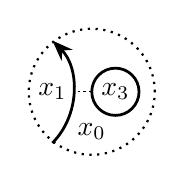
\begin{tikzpicture}[thick,baseline=(current bounding box.center)]

% Dotted circle
\draw[dotted,thick] (0,0) circle (0.8cm);

% Central dotted edge
\draw[dotted, dash pattern=on 1pt off 1pt, line width=0.5pt] (-0.18,0) -- (0.0,0);

% THin edge and circle
\draw[line width=1pt, -Stealth]
  (-0.5,-0.65) .. controls (-0.15,-0.3) and (-0.15,0.3) .. (-0.5,0.65); % edge
\draw[line width=1pt] 
    (0.3,0) circle (0.3cm);   %  circle


% Labels for regions
\node at (0,-0.5) {$x_0$};
\node at (-0.5,0) {$x_1$};
\node at (0.3,0) {$x_3$};

\end{tikzpicture}
}
\newcommand{\ThinEdgeAndCircle}[3]{
\begin{tikzpicture}[thick,baseline=(current bounding box.center)]

% Dotted circle
\draw[dotted,thick] (0,0) circle (0.8cm);

% Central dotted edge
\draw[dotted, dash pattern=on 1pt off 1pt, line width=0.5pt] (-0.18,0) -- (0.0,0);

% THin edge and circle
\draw[line width=1pt, -Stealth]
  (-0.5,-0.65) .. controls (-0.15,-0.3) and (-0.15,0.3) .. (-0.5,0.65); % edge
\draw[line width=1pt] 
    (0.3,0) circle (0.3cm);   %  circle


% Labels for regions
\node at (0,-0.5) {$#1$};
\node at (-0.5,0) {$#2$};
\node at (0.3,0) {$#3$};

\end{tikzpicture}
}

\newcommand{\SingleEdge}[2]{
\begin{tikzpicture}[thick,baseline=(current bounding box.center)]

% Dotted circle
\draw[dotted,thick] (0,0) circle (0.8cm);


% Thin edge and circle
\draw[line width=1pt, -Stealth]
  (-0.5,-0.65) .. controls (-0.15,-0.3) and (-0.15,0.3) .. (-0.5,0.65); % edge


% Labels for regions
\node at (0,-0.5) {$#1$};
\node at (0.3,0) {$#2$};

\end{tikzpicture}
}

\newcommand{\ThickEdgeAndCircleStandard}{
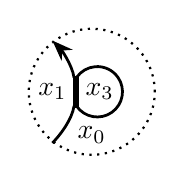
\begin{tikzpicture}[thick,baseline=(current bounding box.center)]

% Dotted circle
\draw[dotted,thick] (0,0) circle (0.8cm);

% Central thick edge
\draw[line width=2.5pt] (-0.2,-0.2) -- (-0.2,0.2);

% THin edge and circle
\draw[line width=1pt,]
  (-0.5,-0.65) .. controls (-0.4,-0.55) and (-0.25,-0.35) .. (-0.225,-0.18); % bottom left
\draw[line width=1pt, -Stealth]
 (-0.225,0.18)  .. controls (-0.25,0.35) and (-0.4,0.55) .. (-0.5,0.65); % top left
\draw[line width=1pt] ([shift=(-145:0.32cm)]0.07,0) arc (-145:145:0.32cm); %circle


% Labels for regions
\node at (0,-0.55) {$x_0$};
\node at (-0.5,0) {$x_1$};
\node at (0.1,0) {$x_3$};

\end{tikzpicture}
}
\newcommand{\ThickEdgeAndCircle}[3]{
\begin{tikzpicture}[thick,baseline=(current bounding box.center)]

% Dotted circle
\draw[dotted,thick] (0,0) circle (0.8cm);

% Central thick edge
\draw[line width=2.5pt] (-0.2,-0.2) -- (-0.2,0.2);

% THin edge and circle
\draw[line width=1pt,]
  (-0.5,-0.65) .. controls (-0.4,-0.55) and (-0.25,-0.35) .. (-0.225,-0.18); % bottom left
\draw[line width=1pt, -Stealth]
 (-0.225,0.18)  .. controls (-0.25,0.35) and (-0.4,0.55) .. (-0.5,0.65); % top left
\draw[line width=1pt] ([shift=(-145:0.32cm)]0.07,0) arc (-145:145:0.32cm); %circle


% Labels for regions
\node at (0,-0.55) {$#1$};
\node at (-0.5,0) {$#2$};
\node at (0.1,0) {$#3$};

\end{tikzpicture}
}

\newcommand{\ThinThinStandard}[1]{\begin{tikzpicture}[thick,baseline=(current bounding box.center)]
% Dotted circle
\draw[dotted,thick] (0,0) circle (1cm);

% Thick and thin edge (flipped vertically)
\draw[dotted, dash pattern=on 1pt off 1pt, line width=0.5pt] (-0.25,-0.38) -- (0.25,-0.38);
\draw[dotted, dash pattern=on 1pt off 1pt, line width=0.5pt] (-0.25,0.38) -- (0.25,0.38);

% Four thinner connecting edges (flipped vertically)
 \draw[line width=1pt, -Stealth] plot[smooth, tension=0.7] coordinates {(-0.5,-0.87) (-0.25,-0.4) (-0.3,0) (-0.25,0.4) (-0.5,0.87)}; %left
  \draw[line width=1pt, -Stealth] plot[smooth, tension=0.7] coordinates {(0.5,-0.87) (0.25,-0.4) (0.3,0) (0.25,0.4) (0.5,0.87)}; %right

% Labels for regions
\node at (0,0) {$#1$};
\node at (0,0.65) {$x_0$};
\node at (-0.65,0) {$x_1$};
\node at (0,-0.65) {$x_2$};
\node at (0.65,0) {$x_3$};

\end{tikzpicture}}
\newcommand{\ThinThin}[5]{\begin{tikzpicture}[thick,baseline=(current bounding box.center)]
% Dotted circle
\draw[dotted,thick] (0,0) circle (1cm);

% Thin edges
\draw[dotted, dash pattern=on 1pt off 1pt, line width=0.5pt] (-0.25,-0.38) -- (0.25,-0.38);
\draw[dotted, dash pattern=on 1pt off 1pt, line width=0.5pt] (-0.25,0.38) -- (0.25,0.38);

% Four thinner connecting edges (flipped vertically)
 \draw[line width=1pt, -Stealth] plot[smooth, tension=0.7] coordinates {(-0.5,-0.87) (-0.25,-0.4) (-0.3,0) (-0.25,0.4) (-0.5,0.87)}; %left
  \draw[line width=1pt, -Stealth] plot[smooth, tension=0.7] coordinates {(0.5,-0.87) (0.25,-0.4) (0.3,0) (0.25,0.4) (0.5,0.87)}; %right

% Labels for regions
\node at (0,0) {$#1$};
\node at (0,0.65) {$#2$};
\node at (-0.65,0) {$#3$};
\node at (0,-0.65) {$#4$};
\node at (0.65,0) {$#5$};

\end{tikzpicture}}

\newcommand{\UnorientedHorizontalThinEdgeStandard}{
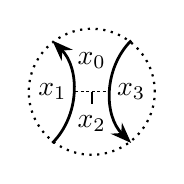
\begin{tikzpicture}[thick,baseline=(current bounding box.center)]

% Dotted circle
\draw[dotted,thick] (0,0) circle (0.8cm);


% Central dotted edge and dash
\draw[dotted, dash pattern=on 1pt off 1pt, line width=0.5pt] (-0.21,0) -- (0.21,0);
\draw[line width=0.75pt] (0,0) -- (0,-0.15);

% Four thinner connecting edges
\draw[line width=1pt, -Stealth]
  (-0.5,-0.65) .. controls (-0.15,-0.3) and (-0.15,0.3) .. (-0.5,0.65); % left
\draw[line width=1pt, Stealth-]
  (0.5,-0.65) .. controls (0.15,-0.3) and (0.15,0.3) .. (0.5,0.65);   %  right


% Labels for regions
\node at (0,0.4) {$x_0$};
\node at (-0.5,0) {$x_1$};
\node at (0,-0.4) {$x_2$};
\node at (0.5,0) {$x_3$};


\end{tikzpicture}
}
\newcommand{\UnorientedHorizontalThinEdge}[5]{
	\begin{tikzpicture}[thick,baseline=(current bounding box.center)]
		
		% Dotted circle
		\draw[dotted,thick] (0,0) circle (0.8cm);
		
		
		% Central dotted edge and dash
		\draw[dotted, dash pattern=on 1pt off 1pt, line width=0.5pt] (-0.21,0) -- (0.21,0);
		\draw[line width=0.75pt] (0,0) -- (0,#5 0.15);
		
		% Four thinner connecting edges
		\draw[line width=1pt, -Stealth]
		(-0.5,-0.65) .. controls (-0.15,-0.3) and (-0.15,0.3) .. (-0.5,0.65); % left
		\draw[line width=1pt, Stealth-]
		(0.5,-0.65) .. controls (0.15,-0.3) and (0.15,0.3) .. (0.5,0.65);   %  right
		
		
		% Labels for regions
		\node at (0,0.4) {$#1$};
		\node at (-0.5,0) {$#2$};
		\node at (0,-0.4) {$#3$};
		\node at (0.5,0) {$#4$};
		
		
	\end{tikzpicture}
}

\newcommand{\UnorientedVerticalThinEdgeStandard}{
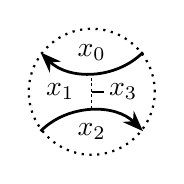
\begin{tikzpicture}[thick,baseline=(current bounding box.center)]

% Dotted circle 
\draw[dotted,thick] (0,0) circle (0.8cm);

% Central dotted edge and dash
\draw[dotted, dash pattern=on 1pt off 1pt, line width=0.5pt] (0,-0.21) -- (0,0.21);
\draw[line width=0.75pt] (0,0) -- (0.15,0);

% Four thinner connecting edges 
\draw[line width=1pt, -Stealth]
 (-0.65,-0.5) .. controls (-0.3,-0.15) and (0.3,-0.15) .. (0.65,-0.5); % bottom
\draw[line width=1pt, Stealth-]
(-0.65,0.5) .. controls (-0.3,0.15) and (0.3,0.15) .. (0.65,0.5);% top


% Labels for regions 
\node at (0.4,0) {$x_3$}; %right
\node at (0,-0.5) {$x_2$}; %bottom
\node at (-0.4,0) {$x_1$}; %left
\node at (0,0.5) {$x_0$}; %top

\end{tikzpicture}
}
\newcommand{\UnorientedVerticalThinEdge}[5]{
	\begin{tikzpicture}[thick,baseline=(current bounding box.center)]
		
		% Dotted circle 
		\draw[dotted,thick] (0,0) circle (0.8cm);
		
		% Central dotted edge and dash 
		\draw[dotted, dash pattern=on 1pt off 1pt, line width=0.5pt] (0,-0.21) -- (0,0.21);
		\draw[line width=0.75pt] (0,0) -- (#5 0.15,0);
		
		% Four thinner connecting edges 
		\draw[line width=1pt, -Stealth]
		(-0.65,-0.5) .. controls (-0.3,-0.15) and (0.3,-0.15) .. (0.65,-0.5); % bottom
		\draw[line width=1pt, Stealth-]
		(-0.65,0.5) .. controls (-0.3,0.15) and (0.3,0.15) .. (0.65,0.5);% top
		
		
		% Labels for regions 
		\node at (0.4,0) {$#4$}; %right
		\node at (0,-0.5) {$#3$}; %bottom
		\node at (-0.4,0) {$#2$}; %left
		\node at (0,0.5) {$#1$}; %top
		
	\end{tikzpicture}
}

\newcommand{\ThinRThickLThickRStandard}[1]{
\begin{tikzpicture}[thick,baseline=(current bounding box.center)]

% Dotted circle 
\draw[dotted,thick] (0,0) circle (1cm);

% thin and thick edges
\draw[dotted, dash pattern=on 1pt off 1pt, line width=0.5pt] (0.1,0.35) -- (0.4,0.35);
\draw[line width=2.5pt] (-0.25,-0.15) -- (-0.25,0.15);
\draw[line width=2.5pt] (0.25,-0.2) -- (0.25,-0.5);

% Connecting edges
\draw[line width=1pt, -Stealth]
 (-0.25,0.13) .. controls (-0.5,0.2) and (-0.65, 0.4) ..  (-0.72,0.72); % top left
\draw[line width=1pt]
 (-0.25,-0.13) .. controls (-0.5,-0.2) and (-0.65, -0.4) ..  (-0.72,-0.72); % bottom left
 \draw[line width=1pt, -Stealth] plot[smooth, tension=0.7] coordinates
 {(-0.25,0.13) (0.1, 0.32) (0.02,0.7) (0,1)}; % top middle
\draw[line width=1pt]
 (0,-1) .. controls (0.05,-0.8) and (0.1, -0.55) ..  (0.25,-0.48); % bottom middle
\draw[line width=1pt,]
  (0.25,-0.48)
  .. controls (0.45,-0.5) and (0.65,-0.65)
  .. (0.72,-0.72); % bottom right
\draw[line width=1pt, smooth, -Stealth, tension=0.7]
  plot coordinates {
    (0.25,-0.22)
    (0.5,0)
    (0.4,0.3) 
    (0.5,0.5)
    (0.72,0.72)
  }; % top right
\draw[line width=1pt]
  (-0.25,-0.13) -- (0.25,-0.22); %internal edge



% Labels for regions 
\node at (0.2,0.05) {$#1$}; 
\node at (-0.25,-0.5) {$x_2$}; 
\node at (-0.7,0) {$x_1$}; 
\node at (-0.25,0.5) {$x_0$};
\node at (0.35,-0.75) {$x_3$}; 
\node at (0.65,-0.3) {$x_4$};
\node at (0.3,0.65) {$x_5$}; 
\end{tikzpicture}
}

\newcommand{\ThickLThickRStandard}{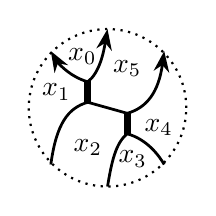
\begin{tikzpicture}[thick,baseline=(current bounding box.center)]

% Dotted circle 
\draw[dotted,thick] (0,0) circle (1cm);

% thick edges
\draw[line width=2.5pt] (-0.25,0.05) -- (-0.25,0.35);
\draw[line width=2.5pt] (0.25,-0.05) -- (0.25,-0.35);

% Connecting edges
\draw[line width=1pt, -Stealth]
 (-0.25,0.33) .. controls (-0.5,0.4) and (-0.65, 0.6) ..  (-0.72,0.72); % top left
\draw[line width=1pt]
 (-0.25,0.07) .. controls (-0.5,0) and (-0.65, -0.2) ..  (-0.72,-0.72); % bottom left
\draw[line width=1pt, Stealth-]
 (0,1) .. controls (-0.05,0.7) and (-0.1, 0.45) ..  (-0.25,0.33); % top middle
\draw[line width=1pt]
 (0,-1) .. controls (0.05,-0.7) and (0.1, -0.45) ..  (0.25,-0.33); % bottom middle
\draw[line width=1pt, ]
 (0.25,-0.33) .. controls (0.5,-0.4) and (0.65, -0.6) ..  (0.72,-0.72); % bottom right
\draw[line width=1pt, -Stealth]
 (0.25,-0.07) .. controls (0.5,0) and (0.65, 0.2) ..  (0.72,0.72); % top right
\draw[line width=1pt]
  (-0.25,0.07) -- (0.25,-0.07); %internal edge



% Labels for regions  
\node at (-0.25,-0.5) {$x_2$}; 
\node at (-0.65,0.2) {$x_1$}; 
\node at (-0.32,0.65) {$x_0$};
\node at (0.32,-0.65) {$x_3$}; 
\node at (0.65,-0.25) {$x_4$};
\node at (0.25,0.5) {$x_5$}; 
\end{tikzpicture}
}

\newcommand{\ThickLThickR}[6]{\begin{tikzpicture}[thick,baseline=(current bounding box.center)]

% Dotted circle 
\draw[dotted,thick] (0,0) circle (1cm);

% thick edges
\draw[line width=2.5pt] (-0.25,0.05) -- (-0.25,0.35);
\draw[line width=2.5pt] (0.25,-0.05) -- (0.25,-0.35);

% Connecting edges
\draw[line width=1pt, -Stealth]
 (-0.25,0.33) .. controls (-0.5,0.4) and (-0.65, 0.6) ..  (-0.72,0.72); % top left
\draw[line width=1pt]
 (-0.25,0.07) .. controls (-0.5,0) and (-0.65, -0.2) ..  (-0.72,-0.72); % bottom left
\draw[line width=1pt, Stealth-]
 (0,1) .. controls (-0.05,0.7) and (-0.1, 0.45) ..  (-0.25,0.33); % top middle
\draw[line width=1pt]
 (0,-1) .. controls (0.05,-0.7) and (0.1, -0.45) ..  (0.25,-0.33); % bottom middle
\draw[line width=1pt, ]
 (0.25,-0.33) .. controls (0.5,-0.4) and (0.65, -0.6) ..  (0.72,-0.72); % bottom right
\draw[line width=1pt, -Stealth]
 (0.25,-0.07) .. controls (0.5,0) and (0.65, 0.2) ..  (0.72,0.72); % top right
\draw[line width=1pt]
  (-0.25,0.07) -- (0.25,-0.07); %internal edge



% Labels for regions  
\node at (-0.25,-0.5) {$#3$}; 
\node at (-0.65,0.2) {$#2$}; 
\node at (-0.32,0.65) {$#1$};
\node at (0.32,-0.65) {$#4$}; 
\node at (0.65,-0.25) {$#5$};
\node at (0.25,0.5) {$#6$}; 
\end{tikzpicture}
}




\newcommand{\ThinThinUnorientedStandard}[1]{\begin{tikzpicture}[thick,baseline=(current bounding box.center)]
% Dotted circle
\draw[dotted,thick] (0,0) circle (1cm);

% Thin edges (coordinates swapped)
\draw[dotted, dash pattern=on 1pt off 1pt, line width=0.5pt] (0.25,0) -- (0.5,0);
\draw[dotted, dash pattern=on 1pt off 1pt, line width=0.5pt] (-0.25,0) -- (-0.5,0);

%thinner connecting edges
\draw[line width=1pt, Stealth-]
(0.8,-0.6) .. controls (0.4,-0.2) and (0.4,0.2)  .. (0.8,0.6);   % left
\draw[line width=1pt, -Stealth]
(-0.8,-0.6) .. controls (-0.4,-0.2) and (-0.4,0.2)  .. (-0.8,0.6);   % lower right

\draw[line width=1pt]
(0,0) circle (0.26cm);   % small circle at center

% Labels for regions (coordinates swapped)
\node at (0,0) {$#1$};
\node at (0.75,0) {$x_3$}; %right
\node at (0,-0.6) {$x_2$}; %down
\node at (-0.75,0) {$x_1$}; %left
\node at (0,0.6) {$x_0$}; %up

		
\end{tikzpicture}}
\newcommand{\ThinThinUnoriented}[5]{\begin{tikzpicture}[thick,baseline=(current bounding box.center)]
		% Dotted circle
		\draw[dotted,thick] (0,0) circle (1cm);
		
		% Thin edges (coordinates swapped)
		\draw[dotted, dash pattern=on 1pt off 1pt, line width=0.5pt] (0.25,0) -- (0.5,0);
		\draw[dotted, dash pattern=on 1pt off 1pt, line width=0.5pt] (-0.25,0) -- (-0.5,0);
		
		%thinner connecting edges
		\draw[line width=1pt, Stealth-]
		(0.8,-0.6) .. controls (0.4,-0.2) and (0.4,0.2)  .. (0.8,0.6);   % left
		\draw[line width=1pt, -Stealth]
		(-0.8,-0.6) .. controls (-0.4,-0.2) and (-0.4,0.2)  .. (-0.8,0.6);   % lower right
		
		\draw[line width=1pt]
		(0,0) circle (0.26cm);   % small circle at center
		
		% Labels for regions (coordinates swapped)
		\node at (0,0) {$#1$};
		\node at (0.75,0) {$#5$}; %right
		\node at (0,-0.6) {$#4$}; %down
		\node at (-0.75,0) {$#3$}; %left
		\node at (0,0.6) {$#2$}; %up
		
		
\end{tikzpicture}}

\newcommand{\ThickThinUnoriented}[5]{\begin{tikzpicture}[thick,baseline=(current bounding box.center)]
		
		
% Dotted circle
\draw[dotted,thick] (0,0) circle (1cm);

% Thin edge and thick edge
\draw[dotted, dash pattern=on 1pt off 1pt, line width=0.5pt] (0.25,0) -- (0.5,0);
\draw[line width=2.5pt] (-0.33,-0.15) -- (-0.33,0.15);

%thinner connecting edges
\draw[line width=1pt, Stealth-]
(0.8,-0.6) .. controls (0.4,-0.2) and (0.4,0.2)  .. (0.8,0.6);   % left
\draw[line width=1pt, smooth, -Stealth, tension=0.8]
plot coordinates {
(-0.8,-0.6)
	(-0.4,0.-0.15)
	(0,-0.26)
(0.25,0) 
(0,0.26)
	(-0.4,0.15)
(-0.8,0.6)
};


% Labels for regions (coordinates swapped)
\node at (0,0) {$#1$};
\node at (0.75,0) {$#5$}; %right
\node at (0,-0.6) {$#4$}; %down
\node at (-0.75,0) {$#3$}; %left
\node at (0,0.6) {$#2$}; %up
		
\end{tikzpicture}}
\newcommand{\ThickThinUnorientedStandard}[1]{\begin{tikzpicture}[thick,baseline=(current bounding box.center)]
		
		
		% Dotted circle
		\draw[dotted,thick] (0,0) circle (1cm);
		
		% Thin edge and thick edge
		\draw[dotted, dash pattern=on 1pt off 1pt, line width=0.5pt] (0.25,0) -- (0.5,0);
		\draw[line width=2.5pt] (-0.33,-0.15) -- (-0.33,0.15);
		
		%thinner connecting edges
		\draw[line width=1pt, Stealth-]
		(0.8,-0.6) .. controls (0.4,-0.2) and (0.4,0.2)  .. (0.8,0.6);   % left
		\draw[line width=1pt, smooth, -Stealth, tension=0.8]
		plot coordinates {
			(-0.8,-0.6)
			(-0.4,0.-0.15)
			(0,-0.26)
			(0.25,0) 
			(0,0.26)
			(-0.4,0.15)
			(-0.8,0.6)
		};
		
		
		% Labels for regions (coordinates swapped)
		\node at (0,0) {$#1$};
		\node at (0.75,0) {$x_3$}; %right
		\node at (0,-0.6) {$x_2$}; %down
		\node at (-0.75,0) {$x_1$}; %left
		\node at (0,0.6) {$x_0$}; %up
		
\end{tikzpicture}}

\newcommand{\ThinThickUnorientedStandard}[1]{\begin{tikzpicture}[thick,baseline=(current bounding box.center)]
		% Dotted circle
		\draw[dotted,thick] (0,0) circle (1cm);
		
		% Thin edge and thick edge
		\draw[dotted, dash pattern=on 1pt off 1pt, line width=0.5pt] (-0.25,0) -- (-0.5,0);
		\draw[line width=2.5pt] (0.33,-0.15) -- (0.33,0.15);
		
		%thinner connecting edges
		\draw[line width=1pt, -Stealth]
		(-0.8,-0.6) .. controls (-0.4,-0.2) and (-0.4,0.2)  .. (-0.8,0.6);   % left
		\draw[line width=1pt, smooth, Stealth-, tension=0.8]
		plot coordinates {
			(0.8,-0.6)
			(0.4,0.-0.15)
			(0,-0.26)
			(-0.25,0) 
			(0,0.26)
			(0.4,0.15)
			(0.8,0.6)
		};
		
		
		% Labels for regions (coordinates swapped)
		\node at (0,0) {$#1$};
		\node at (0.75,0) {$x_3$}; %right
		\node at (0,-0.6) {$x_2$}; %down
		\node at (-0.75,0) {$x_1$}; %left
		\node at (0,0.6) {$x_0$}; %up
		
\end{tikzpicture}}
\newcommand{\ThinThickUnoriented}[5]{\begin{tikzpicture}[thick,baseline=(current bounding box.center)]
		% Dotted circle
		\draw[dotted,thick] (0,0) circle (1cm);
		
		% Thin edge and thick edge
		\draw[dotted, dash pattern=on 1pt off 1pt, line width=0.5pt] (-0.25,0) -- (-0.5,0);
		\draw[line width=2.5pt] (0.33,-0.15) -- (0.33,0.15);
		
		%thinner connecting edges
		\draw[line width=1pt, -Stealth]
		(-0.8,-0.6) .. controls (-0.4,-0.2) and (-0.4,0.2)  .. (-0.8,0.6);   % left
		\draw[line width=1pt, smooth, Stealth-, tension=0.8]
		plot coordinates {
			(0.8,-0.6)
			(0.4,0.-0.15)
			(0,-0.26)
			(-0.25,0) 
			(0,0.26)
			(0.4,0.15)
			(0.8,0.6)
		};
		
		
		% Labels for regions (coordinates swapped)
		\node at (0,0) {$#1$};
		\node at (0.75,0) {$#5$}; %right
		\node at (0,-0.6) {$#4$}; %down
		\node at (-0.75,0) {$#3$}; %left
		\node at (0,0.6) {$#2$}; %up
		
\end{tikzpicture}}



% Theorem-like environments
\usepackage{amsthm}

% Define theorem styles
\theoremstyle{plain} % For theorems, lemmas, propositions
\newtheorem{theorem}{Theorem}[section]
\newtheorem{lemma}[theorem]{Lemma}
\newtheorem{proposition}[theorem]{Proposition}
\newtheorem{corollary}[theorem]{Corollary}

\theoremstyle{definition} % For definitions, examples
\newtheorem{definition}[theorem]{Definition}
\newtheorem{example}[theorem]{Example}

\theoremstyle{remark} % For remarks, notes
\newtheorem{remark}[theorem]{Remark}
\newtheorem{note}[theorem]{Note}



\title{Invariance of Bar-Natan matrix multifactorizations up to 1-homotopy equivalence}
\author{Tomas Mejia Gomez}

\begin{document}


\maketitle

\begin{abstract}
We verify link invariance of a certain construction using matrix factorizations over $\Z[H]$.

\end{abstract}



\section{The construction}

Let $\DD_0$ be a dotted edge and $\DD_1$ be a thick edge. 

Consider a base ring $\KK$ (e.g. $\KK=\Z[\G]$ with grading
$\gr(\G)=i^{-2}h^0q^{-2}$). Take some potential
$P(X)\in \KK[X]$ (or even $\KK [\![X]\!]$ if $\KK$ is big enough). 

We denote by $x_0$, $x_1$, $x_2$ and $x_3$ the variables of surrounding faces, starting above and going counterclockwise. In $\KK[x_0-x_1,x_2-x_1,x_3-x_2]$, it is always possible to factor
$$W=P(x_0-x_1)+P(x_3-x_0)-P(x_2-x_1)-P(x_3-x_2)= (x_0-x_2)(x_0+x_2-x_1-x_3)Z$$
for some $Z=Z(x_0-x_1,x_2-x_1,x_3-x_2)\in \KK[x_0-x_1,x_2-x_1,x_3-x_2]$. We often drop the inputs of $Z$ to lighten notation.


We assign Koszul matrix factorizations
\begin{align*}
    M(\DD_0)&=K(x_0-x_2,\quad (x_0+x_2-x_1-x_3)Z)\\
    M(\DD_1)&=K(Z,\quad (x_0-x_2)(x_0+x_2-x_1-x_3)).
\end{align*}

Given two matrix factorizations of the form
$$M=[\mfshort{  A}{\hslash B}{}{}],\qquad M'=[\mfshort{A'}{\hslash  B'}{}{}],$$
with $A,A',B$ and $B'$ concentrated in $\hslash$-degree 0, we often specify morphisms by spelling out their components in each $\hslash$-degree as follows:
\[
\begin{tikzcd}
    M \arrow[d, "{\hslash^0(\alpha,\beta)}",swap] \\ M'
\end{tikzcd}
=
\begin{tikzcd}
    {} [ \: A \arrow[d, "\alpha", shift left=3pt]\arrow[r, out=5, in=175, bend left=10]  &  \hslash B\:]\arrow[d, "\beta", shift right=1pt] \arrow[l, out=185, in=-5, swap]\\
   {}  [\:A' \arrow[r, out=5, in=175, bend left=10]& 
    \hslash B' \arrow[l, out=185, in=-5, swap]\:]
\end{tikzcd}\qquad\qquad 
\begin{tikzcd}
    M \arrow[d, "{\hslash^1(\alpha,\beta)}",swap] \\ M'
\end{tikzcd}
=
\begin{tikzcd}
    {}  [\:A \arrow[dr, "\alpha"{pos=1}, out=-45, in=120]\arrow[r, out=5, in=175, bend left=10]  &  \hslash B\:]\arrow[dl, "\beta"{pos=1}, out=-135, in=60,swap] \arrow[l, out=185, in=-5, swap]\\
     {} [\:A' \arrow[r, out=5, in=175, bend left=10]& 
     \hslash B' \arrow[l, out=185, in=-5, swap]\:]
\end{tikzcd}
\]
Many useful maps can be easily expressed in this notation. For instance, the differential $d_M:M\to M$ itself takes the form
$$d_m=\hslash^1 (d_0,d_1)$$
In the case $M'=\hslash M$ we use the special notation
$$s_\hslash =\hslash^1(1,1):M\to \hslash M$$

For Koszul matrix factorizations, we will take the convention
$$K_{R}(a\sc b)=\mfshort{q^{\deg_q(a)+3}R}{ \hslash R}{a}{b}.$$

Here, the grading $\hslash$ is a $\Z/2$ grading. A shift $\hbar M$ on a matrix factorization $M$ has the additional effect of switching the sign of all differentials. This helps us keep track of Koszul sign rules for tensor products of matrix factorizations. Namely, if we tensor a Koszul factorization $K_{R}(a\sc b)$ with some other matrix factorization $M$, we can write
$$K_{R}(a\sc b)\otimes M =\left[ \mfshort{q^{\deg_q(a)+3}M}{\hslash M}{a}{b} \right],$$
which indicates that the tensor product splits, as free $R$-module, into two copies of $M$, with the first one shifted in $q$ and $\hslash$ degrees. In terms of this decomposition, the total differential takes the form
$$d_{K_{R}(a\sc b)\otimes M} = \begin{pmatrix}
    d_M & b \\ a & -d_M
\end{pmatrix},$$
where the negative sign comes precisely from the $\hslash$-shift. Observe also that here $a$ and $b$ are understood to have $\hslash$-degree 1, and they could be more explicitly denoted by $\hslash^1(a,a)$ and $\hslash^1(b,b)$, respectively.

If we want to switch the sign of differentials without altering the $\hslash$ degree, we write $-M$. Using these notations, we have \todo{not sure if I need this}
\begin{align*}
    \hbar (M\otimes N) &= (\hbar M)\otimes N = (-M)\otimes(\hbar N)
\end{align*}


% Then define for a positive crossing $\DD_+$ and a negative crossing $\DD_-$ the multifactorizations
% $$M(\DD_+)=\left[i^1M(\DD_0)\longrightarrow i^{-1}h^1M(\DD_1) \right],\qquad M(\DD_-)=\left[i^1h^{-1}M(\DD_1)\longrightarrow i^{-1}M(\DD_0) \right]$$
% as mapping cones of the canonical zip/unzip maps.

The most general webs we will be dealing with can be obtained by taking an oriented planar arc diagram $T$ where all inputs have exactly two consecutive incoming arcs and two consecutive outgoing arcs, and then plugging $\DD_0$ or $\DD_1$ in each input while respecting orientations:
$$\DD=T(\DD_{i_1},\dots,\DD_{i_k}),$$ 
with $i_j=0$ or $1$.

\section{Hom spaces}

Given two webs $\DD_1$ and $\DD_2$ with the same boundary, we want a good handle of the space $$Hom(M(\DD_2),M(\DD_1)).$$

First, we need to understand closed webs. Let $\DD$ be a closed web

When we glue the mirror $\DD_1$ and the mirror $\overline\DD_2$ along the boundary, we obtain a closed web denoted $\DD_1\cup \overline\DD_2$



\begin{lemma}
$$\Ext(M(\DD_2),M(\DD_1))\cong H(M(\DD_1\cup \overline\DD_2))$$
\end{lemma}

\begin{proposition}

\end{proposition}

\section{Invariance}

The invariance of $M(D)$ for a link diagram $D$ under each Reidemeister move will proceed by looking at the explicit matrix multifactorization associated to the relevant local piece of the diagram and simplifying it in two steps. In the first step, one simplifies each resolving web into smaller webs with no internal faces, and then extends into a special 0-deformation retract of the entire multifactorization. There is enough control of the deformation data to compute explicit differentials in the resulting multifactorization, and in particular to identify some identity components in $d_1$. The second step then consists of simplifying along such identities to obtain a special 1-deformation retract into the desired form.

Reidemeister I moves are illustrated in Figure \ref{fig:R1}. The purple arrows represent special deformation retracts of vertical matrix factorizations, where each component is obtained from Lemma \ref{lemma:sdrkoszullinear} or Lemma $\ref{lemma:sdrkoszul}$. We then extend, by Lemma \ref{specialDefRetract}, to a special 0-deformation retract of multifactorizations. Notice that we indicate the explicit form of the $d_1$-component in each of the once-simplified multifactorizations. These are computed as composites:
\[
\begin{tikzcd}[column sep=2cm,ampersand replacement=\&]
q^2\scalebox{0.5}{\SingleEdge{}{}}\oplus \scalebox{0.5}{\SingleEdge{}{}}   
\arrow[r, "{\begin{pmatrix} \hslash^0(1,0)&\hslash^0(x_3-x_0,0)
\end{pmatrix}}"] 
\&[1.2cm]
q\hslash\scalebox{0.5}{\ThinEdgeAndCircle{}{}{}} 
\arrow[r, "{\hslash^1(1,2x_0-x_1-x_3)}"]
\&
q^2h\scalebox{0.5}{\ThickEdgeAndCircle{}{}{}}
\arrow[r, "{\hslash^0(0,P^0_{f(y)})}", "\scalebox{0.6}{$\begin{matrix}
    y=x_3-x_0 \\ f(y)= x_3-x_0
\end{matrix}$}"']
\&[-0.4cm]
q^2h\hslash\scalebox{0.5}{\SingleEdge{}{}} 
\end{tikzcd}
\]
\[
\begin{tikzcd}[column sep=2cm, ampersand replacement=\&]
q^{-2}h^{-1}\hslash\scalebox{0.5}{\SingleEdge{}{}}  
\arrow[r, "{\hslash^0(0,1)}"] 
\&[-1.2cm]
q^{-2}h^{-1}\hslash\scalebox{0.5}{\ThickEdgeAndCircle{}{}{}}
\arrow[r, "{\hslash^1(1,2x_0-x_1-x_3)}"]
\&
q^{-1}\scalebox{0.5}{\ThinEdgeAndCircle{}{}{}} 
\arrow[r, "{\begin{pmatrix} \hslash^0(P^0_{f(y)},0) \\
\hslash^0(P^1_{f(y)},0) \end{pmatrix}}", "\scalebox{0.6}{$\begin{matrix}
    y=x_3-x_0 \\ f(y)= (2x_0-x_1-x_3)((x_3-x_1)-H)
\end{matrix}$}"']
\&
\scalebox{0.5}{\SingleEdge{}{}}\oplus q^{-2}\scalebox{0.5}{\SingleEdge{}{}}
\end{tikzcd}
\]



The summands 
$$
q^2\scalebox{0.5}{\SingleEdge{}{}}
\xrightarrow{\hslash^1(1,0)} 
q^2\hslash h\scalebox{0.5}{\SingleEdge{}{}},
\qquad \qquad 
q^{-2}\hslash h^{-1}\scalebox{0.5}{\SingleEdge{}{}}
\xrightarrow{\hslash^1(0,-1)} 
q^{-2}\scalebox{0.5}{\SingleEdge{}{}}
$$
are easily verified to be 1-contractible. The corresponding special 1-deformation retractions cancelling these summands are represented by the green arrows.


\begin{figure}
    \centering
\[\label{r1}
\begin{tikzcd}[column sep=1.8cm, ampersand replacement=\&]
\scalebox{0.7}{\SingleEdge{}{}}  
\arrow[d, color=ForestGreen, shift right=1.5] 
\& \\
q^2\scalebox{0.7}{\SingleEdge{}{}}\oplus \scalebox{0.7}{\SingleEdge{}{}}  
\arrow[u, color=ForestGreen, shift right=1.5] 
\arrow[d, color=violet, shift right=1.5] 
\arrow[r, "{\begin{pmatrix}\hslash^1(1,0) & \hslash^1(x_1-x_0,0) \end{pmatrix}}", shift left=3, bend left=20, start anchor=east, end anchor=west]
\&
q^2\hslash h\scalebox{0.7}{\SingleEdge{}{}} 
\arrow[d, color=violet, shift right=1.5]
\arrow[l, color=ForestGreen, shift left=1]
\\
q\scalebox{0.7}{\ThinEdgeAndCircle{}{}{}} \arrow[r]
\arrow[u, color=violet, shift right=1.5] 
\arrow[loop right, distance=1.5em, in=-75, out=-105, color=violet]
\&
q^2\hslash h\scalebox{0.7}{\ThickEdgeAndCircle{}{}{}} 
\arrow[u, color=violet, shift right=1.5] 
\arrow[loop right, distance=1.5em, in=-75, out=-105, color=violet] 
\end{tikzcd} 
\quad
\begin{tikzcd}[column sep=1.8cm]
 & 
 \scalebox{0.7}{\SingleEdge{}{}}  
 \arrow[d, color=ForestGreen, shift right=1.5] 
 \\
q^{-2}h^{-1}\hslash\scalebox{0.7}{\SingleEdge{}{}}   \arrow[d, color=violet, shift right=1.5] 
\ar[r, "{\begin{pmatrix}\hslash^1(0,x_0-x_1) \\\hslash^1(0,-1)
\end{pmatrix}}", shift left=1] 
&
\scalebox{0.7}{\SingleEdge{}{}}\oplus q^{-2}\scalebox{0.7}{\SingleEdge{}{}} 
\arrow[d, color=violet, shift right=1.5]
\arrow[u, color=ForestGreen, shift right=1.5] 
\ar[l, color=ForestGreen, shift left=1] 
\\
q^{-2}\hslash h^{-1}\scalebox{0.7}{\ThickEdgeAndCircle{}{}{}} 
\ar[r] 
\arrow[u, color=violet, shift right=1.5] 
\arrow[loop right, distance=1.5em, in=-75, out=-105, color=violet] 
&
q^{-1}\scalebox{0.7}{\ThinEdgeAndCircle{}{}{}} 
\arrow[u, color=violet, shift right=1.5] 
\arrow[loop right, distance=1.5em, in=-75, out=-105, color=violet]
\end{tikzcd}
\]
    \caption{Invariance under positive and negative Reidemeister I moves}
    \label{fig:R1}
\end{figure}

Concerning Reidemeister 2, here is what we do now

\[\label{r2sdr}
\begin{tikzcd}[row sep=-0.1cm, column sep=3cm]
& 
\scalebox{0.7}{\ThinEdge{}{}{}{}}
\arrow[dr]
\arrow[ddd, bend left=40, color=violet, shift right=1.5, dash pattern=on 40pt off 35pt]
\arrow[leftarrow, ddd, bend left=40, color=violet, shift left=1.5, dash pattern=on 39.5pt off 37pt]
&
\\
q^{-1}h^{-1}\hslash\scalebox{0.7}{\ThickEdge{}{}{}{}} 
\arrow[dr]
\arrow[ur]
\arrow[ddd, color=violet, shift right=1.5]
&
&
qh\hslash\scalebox{0.7}{\ThickEdge{}{}{}{}}
\arrow[ddd, color=violet, shift right=1.5]
\\
& 
q\scalebox{0.7}{\ThickEdge{}{}{}{}}\oplus q^{-1}\scalebox{0.7}{\ThickEdge{}{}{}{}}
\arrow[ur, crossing over] 
&
\\[2em]
& 
\scalebox{0.7}{\ThinThin{}{}{}{}{}}
\arrow[loop right, distance=1.5em, in=-75, out=-105, color=violet]
\arrow[dr]
&
\\
q^{-1}h^{-1}\hslash\scalebox{0.7}{\ThinThick{}{}{}{}{}} 
\arrow[loop right, distance=1.5em, in=-75, out=-105, color=violet]
\arrow[ur]
\arrow[dr]
\arrow[uuu, color=violet, shift right=1.5]
&& 
qh\hslash\scalebox{0.7}{\ThinThick{}{}{}{}{}}
\arrow[uuu, color=violet, shift right=1.5]
\arrow[loop right, distance=1.5em, in=-75, out=-105, color=violet]
\\
& 
\scalebox{0.7}{\Bigon{}{}{}{}{}} 
\arrow[ur]
\arrow[loop right, distance=1.5em, in=-75, out=-105, color=violet] 
&
\arrow[ddd, from=3-2, to=6-2, bend right=40, crossing over, color=violet, shift right=1.5] 
\arrow[uuu, from=6-2, to=3-2, bend left=40, crossing over, color=violet, shift right=1.5] 
\arrow[ur, from=3-2, to=2-3, crossing over] 
\arrow[rr, from=2-1, to=2-3, crossing over] 
\end{tikzcd}
\]


\begin{definition}
Let $(C,D)$ and $(C',D')$ be multifactorizations. Then a special $n$-deformation retract from $C$ to $C'$ consists of 0-morphisms $P:C\to C'$ and $I:C'\to C$ such that $PI=1$, together with a $n$-homotopy $H:C\to C$ between $1$ and $IP$ such that $HI=0$, $PH=0$ and $H^2=0$. We represent all this data by
$$\sdr{(C',D')}{(C,D)}{I}{P}{H}$$
\end{definition}

The next lemma tells us how to simplify certain Koszul matrix factorizations into special deformation retracts.

\begin{lemma}\label{sdrlemma}    (Adapted from KR \textcolor{red}{How general is $R$?}) Let $R$ be an integral domain. Let $\overline W\in R$ and $f,g\in R[y]$ so that $f$ has the form $f=uy^n+\tilde f$ wtih $u\in R[y]^\times$ and $\deg_y(\tilde f)<n$. Let $M$ be a matrix factorization over $R[y]$ with potential $W=\overline W-fg\in R[y]$. Let 
\begin{align*}M'&=M/fM,\\
\overline M &= K_{R[y]}(f;g)\otimes_{R[y]} M,\end{align*}
thought of as matrix factorizations over $R$ with potential $\overline W$.
Then there is a strong deformation retract
$$\sdr{M'}{\overline M}{I}{P}{H}$$
of the form
 $$\begin{tikzcd}[column sep=large, ]
    &M/fM\ar[dd, shift right=0.6ex, "I_v", swap]\ar[dd, leftarrow, shift left=0.6ex, "P"]\arrow[ddl, "I_d", bend right=20, swap]\\\\
    q^{3-2n}\hslash M\arrow[r, "f", shift left=0.5ex, bend left=20]& M\ar[l, "H"]\arrow[l, "g", shift left=0.5ex, bend left=20], 
\end{tikzcd}$$
The arrows are as follows:
\begin{itemize}
    \item $P$ is the usual projection.
    \item $H=-\Quo_f$, the negative of the quotient of division by $f$.
    \todo{carry the modification of the sign of $H$}
    \item $I$ consists of a vertical component $I_v=\Res_f$ given by the residue of division by $f$, and a diagonal component $I_d$ given by the composite $H\circ d_M\circ I_v$.
\end{itemize}
\end{lemma}


In many cases of interest, we additionally have decompositions $M/fM=\bigoplus_{i=0}^{k}M_i$ as matrix factorizations over $R$. Such an identification, in conjunction with the lemma, will then produce a special deformation retract that simplifies $M$ into a sum of simpler matrix factorizations over a ring with one less variable.

The following is a straightforward corollary.

\begin{lemma}\label{lemma:sdrkoszullinear}
    In the set up of Lemma \ref{sdrlemma}, assume that $M=K_{R[y]}(\mathbf{\overline a},\mathbf{\overline b})$
    and that 
    $f=y-f_0$, where $\deg_y(f_0)=0$. Then, under the identification 
    $M/yM\cong K_{R}\left(\left.\mathbf{\overline a}\right|_{y=f_0},\left.\mathbf{\overline b}\right|_{y=f_0}\right)$,
    we have a special deformation retract
     $$
\begin{tikzcd}[column sep=large]
    &
    K_{R}\left(\left.\mathbf{\overline a}\right|_{y=f_0},\left.\mathbf{\overline b}\right|_{y=f_0}\right)
    \ar[dd, shift right=0.6ex, "1", swap]
    \ar[dd, leftarrow, shift left=0.6ex, "y\mapsto f_0"]
    \arrow[ddl, "{}", bend right=20, swap]
    \\\\
    q\hslash K_{R[y]}(\mathbf{\overline a},\mathbf{\overline b})
    \arrow[r, "f", shift left=0.5ex, bend left=20]
    & 
    K_{R[y]}(\mathbf{\overline a},\mathbf{\overline b})
    \ar[l, "-\Quo_f"]
    \arrow[l, "g", shift left=0.5ex, bend left=20], 
\end{tikzcd}
$$
The diagonal component of the inclusion is the composite
$$
\begin{tikzcd}
    K_{R}\left(\left.\mathbf{\overline a}\right|_{y=f_0},\left.\mathbf{\overline b}\right|_{y=f_0}\right) \arrow[r, "{\sum_{j=1}^k1\otimes\cdots \otimes\hslash^1(-\Quo_f\circ a_j,-\Quo_f\circ b_j)\otimes\cdots\otimes 1}"] 
    &[5cm]
    qK_{R[y]}\left(\mathbf{\overline a},\mathbf{\overline b}\right) 
    \arrow[r,"s_\hslash"] 
    & 
    q\hslash K_{R[y]}\left(\mathbf{\overline a},\mathbf{\overline b}\right)
\end{tikzcd}
$$
\end{lemma}

This can be generalized 

\begin{lemma}\label{lemma:sdrkoszul}\todo{that final degree switch in $\hslash$}
    In the set up of Lemma \ref{sdrlemma}, assume that $M=K_{R[y]}(\mathbf{\overline a},\mathbf{\overline b})$ and that $\deg_y(\Res_f(a_i))=\deg_y(\Res_f(b_i))=0$ for all $i$. Then the map
    $$\bigoplus_{i=0}^{n -1} q^{-2i}K_{R}\left(\Res_f\mathbf{\overline a},\Res_f\mathbf{\overline b}\right)\xrightarrow{(y^i)_i}M/fM$$ is an isomorphism of matrix factorizations over $R$ and, combined with Lemma \ref{sdrlemma}, gives a special deformation retract
     $$\begin{tikzcd}[column sep=large, ]
    &\displaystyle\bigoplus_{i=0}^{n -1} q^{-2i}K_{R}\left(\Res_f\mathbf{\overline a},\Res_f\mathbf{\overline b}\right)\ar[dd, shift right=0.6ex, "(y^i)_i", swap]\ar[dd, leftarrow, shift left=0.6ex, "\left(\frac{1}{i!}\left.\frac{\partial^i}{\partial y^i}\right|_{y=0}\circ \Res_f\right)_i"]\arrow[ddl, "{}", bend right=20, swap]\\\\
    q^{3-2n}\hslash K_{R[y]}(\mathbf{\overline a},\mathbf{\overline b})\arrow[r, "f", shift left=0.5ex, bend left=20]& K_{R[y]}(\mathbf{\overline a},\mathbf{\overline b})\ar[l, "\Quo_f"]\arrow[l, "g", shift left=0.5ex, bend left=20], 
\end{tikzcd}$$
The diagonal component of the inclusion is the composite
$$
\begin{tikzcd}
    \displaystyle\bigoplus_{i=0}^{n-1}q^{-2i}K_{R}\left(\Res_f\mathbf{\overline a},\Res_f\mathbf{\overline b}\right) \arrow[r, "{\left(\sum_{j=1}^k1\otimes\cdots \otimes\hslash^1(\Quo_f\circ y^i a_j,\Quo_f\circ y^i b_j)\otimes\cdots\otimes 1\right)_i}"] &[5.5cm] q^{3-2n}K_{R[y]}\left(\mathbf{\overline a},\mathbf{\overline b}\right) \arrow[d,"s_\hslash"] \\& q^{3-2n}\hslash K_{R[y]}\left(\mathbf{\overline a},\mathbf{\overline b}\right)
\end{tikzcd}
$$
\end{lemma}

% It is useful to express the special deformation retract afforded by the lemma using this identification. For this purpose, let us introduce the notation 
% $$T_f^i=\frac{1}{i!}\left.\frac{\partial^i}{\partial y^i}\right|_{y=0}\circ\Res_f:M\to q^{2i}M_R$$
% for the $R$-module map that takes the coefficient of $y^i$ in the residue of division by $f$. These can be bundled together into $T_f: M\to \bigoplus_{i=0}^{n-1}q^{2i} M_R$. With this, we have

% $$\begin{tikzcd}[column sep=large, ]
%     &\bigoplus_{i=0}^{n-1}q^{2i} M_R\ar[dd, shift right=0.6ex, "T_f", swap]\ar[dd, leftarrow, shift left=0.6ex, "T_f"]\arrow[ddl, "H\circ d_M\circ T_f", bend right=20, swap]\\\\
%     M\arrow[r, "f", shift left=0.5ex, bend left=20]& M\ar[l, "\Quo_f"]\arrow[l, "g", shift left=0.5ex, bend left=20], 
% \end{tikzcd}$$

% 
\subsection{MOY moves for rational $\sl_n$}
The following explicit instances of the lemma should be thought of as refinements of MOY moves.

Circle removal:\\

    \begin{minipage}[c]{0.5\textwidth}
        \begin{align*}
            R &= \Q[\G, x_0-x_1] \\
            M &= R[x_3-x_0] \\
            \overline{W} &= 0 \\
            (n+1)(x_3-x_0)^n-p &= (2x_0-x_1-x_3)Z \\
            q &= 0
        \end{align*}
    \end{minipage}
    \hfill
    \begin{minipage}[c]{0.45\textwidth}
        \[\begin{tikzcd}[column sep=3cm]
            \bigoplus_{i=0}^{n-1}R\ar[dd, shift right=0.6ex, swap]\ar[dd, leftarrow, shift left=0.6ex]&\\\\
            R[x_3-x_0]\arrow[r, "0", shift left=0.5ex, bend left=15]& R[x_3-x_0]\ar[l, "H"]\ar[l, "(2x_0-x_1-x_3)Z", shift left=0.5ex, bend left=15]
        \end{tikzcd}\]
    \end{minipage}

    \vspace{1cm} % Adds some vertical space between the items
Loop removal:\\

    \begin{minipage}[c]{0.5\textwidth}
        \begin{align*}
            R&= \Q[\G, x_0-x_1] \\
            M &= R[x_3-x_0]\\
            \overline{W} &= 0 \\
            (n+1)(x_3-x_0)^{n-1}-p &= Z \\
            q &= 0
        \end{align*}
    \end{minipage}
    \hfill
    \begin{minipage}[c]{0.45\textwidth}
        \[\begin{tikzcd}[column sep=3cm]
            &\bigoplus_{i=0}^{n-2}R\ar[dd, shift right=0.6ex, swap]\ar[dd, leftarrow, shift left=0.6ex]\\\\
            R[x_3-x_0]\arrow[r, "Z", shift left=0.5ex, bend left=15]& R[x_3-x_0]\ar[l, "H"]\ar[l, "0", shift left=0.5ex, bend left=15]
        \end{tikzcd}\]
    \end{minipage}

Digon removal:\\
        \begin{align*}
            R&= \Q[\G, x_0-x_1,x_2-x_1,x_3-x_2] \\
            M &= K(Z(x_0-x_1,x-x_1,x_3-x),(x_0-x)(x_0+x-x_1-x_3))_{R[x-x_1]}\\
            \tilde M &= K(Z(x_0-x_1,x_2-x_1,x_3-x_2),(x_0-x_2)(x_0+x_2-x_1-x_3))_{R}\\
            \overline{W} &= P(x_0-x_1)+P(x_3-x_0)-P(x_2-x_1)-P(x_3-x_2) \\
            (x-x_1)^{2}-p &=  (x-x_2)(x+x_2-x_1-x_3)\\
            q &= Z(x-x_1,x_2-x_1,x_3-x_2)
        \end{align*}
       $$\begin{tikzcd}[column sep=3cm]
        \tilde M\oplus \tilde M\ar[dd, shift right=0.6ex, swap]\ar[dd, leftarrow, shift left=0.6ex]&\\\\
            M\ar[r, "{Z(x-x_1, x_2-x_1,x_3-x_2)}", shift left=0.5ex, bend left=15]& M\ar[l, "H"]\ar[l, "(x-x_2)(x+x_2-x_1-x_3)", shift left=0.5ex, bend left=15]
        \end{tikzcd}$$

Square removal:
        \begin{align*}
            R&= \Q[\G, x_0-x_1,x_2-x_1,x_2-x_3] \\
            M &= K(Z(x_0-x_1,x_2-x_1,x-x_2),(x_0-x_2)(x_0+x_2-x_1-x))_{R[x-x_0]}\\
            M_0 &= K()_{R}\\
            M_1 &= K()_{R}\\
            \overline{W} &= P(x_0-x_1)-P(x_0-x_3)-P(x_2-x_1)+P(x_2-x_3) \\
            (n+1)(x-x_0)^{n-1}-p &=  Z(x_2-x_3,x_0-x_3,x-x_0)\\
            q &= (x_2-x_0)(x_2+x_0-x_3-x)
        \end{align*}
       $$\begin{tikzcd}[column sep=3cm]
        &M_0\oplus \bigoplus_{i=0}^{n-3} M_1\ar[dd, shift right=0.6ex, swap]\ar[dd, leftarrow, shift left=0.6ex]\\\\
            M\ar[r, "{Z(x_2-x_3,x_0-x_3,x-x_0)}", shift left=0.5ex, bend left=15]& M\ar[l, "H"]\ar[l, "(x_2-x_0)(x_2+x_0-x_3-x)", shift left=0.5ex, bend left=15]
        \end{tikzcd}$$



\end{document}
\subsection{MOY moves in $\uone$-equivariant $\sl_2$}
The base ring is $\mathbf K=\Z[H]$, and the elementary matrix factorizations are over $R=\mathbf K[x_0-x_1,x_2-x_1,x_3-x_2]$.

\todo{it seems like $H-(x_3-x_1)$ in Caludius' paper has the wrong sign if we want to get the correct potential. I'm swapping the sign}

\begin{align*}
    D_0=\ThinEdgeStandard &\longmapsto M(D_0)=\left[\mf{q\hslash R}{R}{x_0-x_2}{(x_0+x_2-x_1-x_3)((x_3-x_1)-H)}\right]\\
    D_1=\ThickEdgeStandard &\longmapsto M(D_1)=\left[\mf{q R}{\hslash R}{(x_3-x_1)-H}{(x_0+x_2-x_1-x_3)(x_0-x_2)}\right]
\end{align*}\todo{seems like we should swap all the $\hslash$ degrees here. maybe even in the definition of koszul}

When working locally, other boundary orientations are also possible. Thus, we also define
\begin{align*}
D_2=\UnorientedHorizontalThinEdgeStandard &\longmapsto M(D_2)=\left[\mf{q\hslash R}{R}{x_0-x_2}{(x_0+x_2-x_1-x_3-H)(x_3-x_1)}\right]\\
D_3=\UnorientedVerticalThinEdgeStandard &\longmapsto M(D_3)=\left[\mf{q\hslash R}{R}{x_1-x_3}{(x_0+x_2-x_1-x_3-H)(x_2-x_0)}\right]
\end{align*}
Observe that in all three types of thin edges, there is a \emph{negative region} whose variable appears with a negative sign in the linear term of the associated matrix factorization. In the case of $D_2$ and $D_3$ there is a 180 degree rotational symmetry. To avoid ambiguity, we indicate the negative region by a little dash.

\todo{arrows somehow ruin the symmetry of the pics}


The elementary matrix factorizations can be expressed as
\begin{align*}
    M(D_0)&=K_R(x_0-x_2\sc(x_0+x_2-x_1-x_3)((x_3-x_1)-H))\\
    M(D_1)    &= qK_R((x_0+x_2-x_1-x_3)(x_0-x_2)\sc (x_3-x_1)-H)\\
    &=\hslash K_R(H-(x_3-x_1)\sc(x_0+x_2-x_1-x_3)(x_2-x_0))
\end{align*}

Notice that $R$ is the subring of the polynomial ring in all face variables generated by differences across edges. We refer to $R$ as the \emph{edge ring}, and we extend this nomenclature to more general webs in the expected way. The particular case $R=\mathbf K[x_0-x_1,x_2-x_1,x_3-x_2]$ is refered to as the \emph{standard edge ring}. We will often omit the specification of the edge ring when variables are already explicit in the web diagram.



Let us write some explicit special deformation retracts that can be used for computations and proof of invariance. 

\subsection{Thin edge removal}
Lemma \ref{lemma:sdrkoszullinear} can be applied to remove dotted edges that bound an interior region.
\begin{proposition}
Let $D$ be a four-ended web with a thin edge $e$ such that its negative region is interior. Denote the corresponding edge ring by $R_D$, and the variables associated to the positive and negative region of $e$ by $x_+$ and $x_-$, respectively. Let $D'$ be the web obtained by removal of $e$, so that its edge ring $R_{D'}$ no longer involves $x_-$. Then there is a special deformation retract of matrix factorizations over $R_{D'}$
$$\sdr{M(D')}{M(D)}{}{}{}$$ 
of the form
 $$\begin{tikzcd}[column sep=large, ]
    &M(D')\ar[dd, shift right=0.6ex, "1", swap]\ar[dd, leftarrow, shift left=0.6ex, "x_-\mapsto x_+"]\arrow[ddl, "{s_\hslash\circ\sum_{j}1\otimes\cdots \otimes\hslash^1(\Quo_f\circ a_j,\Quo_f\circ b_j)\otimes\cdots\otimes 1}", bend right=20, swap]\\\\
    q\hslash \widetilde M(D)\arrow[r, "f=x_+-x_-", shift left=0.5ex, bend left=20]& \widetilde M(D)\ar[l, "H"]\arrow[l, "g", shift left=0.5ex, bend left=20], 
\end{tikzcd}$$
where $\widetilde M(D)$ is the Koszul factorization over $R_D$ obtained from all edges in $D$ except $e$. The only contributions to the sum come from edges with at least one end adjacent to the $x_-$-region.
\end{proposition}

A similar statement is true if the positive region is interior and the variable $x_+$ is eliminated instead.

Here is an example, which will be of use later.
\[
\begin{tikzcd}[column sep=large, ]
    &\scalebox{0.7}{\ThickLThickRStandard} \ar[dd, shift right=0.6ex, "1", swap]\ar[dd, leftarrow, shift left=0.6ex, "u\mapsto x_5"]\arrow[ddl, "{s_\hslash\circ\left(\hslash^1(-1,x_0-x_2)\otimes 1+1\otimes\hslash^1(0,x_3-u)\right)}", bend right=20, swap]\\\\
    q\hslash \scalebox{0.7}{\ThickLThickR{x_0}{x_1}{x_2}{x_3}{x_4}{u}}[x_5-u]\arrow[r, "x_5-u", shift left=0.5ex, bend left=20]& \scalebox{0.7}{\ThickLThickR{x_0}{x_1}{x_2}{x_3}{x_4}{u}}[x_5-u]\ar[l, "H"]\arrow[l, "(x_5+u-x_0-x_4)((x_4-x_0)-H)", shift left=0.5ex, bend left=20], 
\end{tikzcd}
\]


\subsubsection{Bigon removal}
In the case of bigon removal, we have
\begin{align*}
\BigonStandard{u} &= q^2K_{R[u-x_0]}
    \begin{pmatrix}
    (x_0+u-x_1-x_3)(x_0-u) & (x_3-x_1)-H\\
    (u+x_2-x_1-x_3)(u-x_2) & (x_3-x_1)-H
    \end{pmatrix}
\end{align*}
Letting $y=u-x_0$, $f=(u+x_2-x_1-x_3)(u-x_2)$ and $M=K_{R[u-x_0]}((x_0+u-x_1-x_3)(x_0-u)\sc (x_3-x_1)-H)$, we are under the hypotheses of Lemma \ref{lemma:sdrkoszul}. In particular, we have a strong deformation retract
\[
\begin{tikzcd}[column sep=3cm, row sep=2cm]
    q\scalebox{0.7}{\ThickEdgeStandard}\oplus q^{-1}\scalebox{0.7}{\ThickEdgeStandard} \arrow[d, shift right=2, "{\begin{pmatrix} 1 \quad u-x_0\end{pmatrix}}", swap] \arrow[dr, bend left=20, "{\begin{pmatrix} \hslash^0(-1,0) \quad \hslash^0(x_0-u,0)\end{pmatrix}}"] 
    &\\   q\scalebox{0.7}{\ThickEdge{u}{x_1}{x_2}{x_3}}[u-x_0] \arrow[u, shift right=2, "{\begin{pmatrix} \left.\id\right|_{u=x_0} 
    \\    \left.\frac{\partial}{\partial(u-x_0)}\right|_{u=x_0}\end{pmatrix}\circ\Res_{f}}",swap]\arrow[r, "(x_3-x_1)-H", bend left=5]& \hslash\scalebox{0.7}{\ThickEdge{u}{x_1}{x_2}{x_3}}[u-x_0] \arrow[l, "(x_0+u-x_1-x_3)(x_0-u)", bend left=5]
\end{tikzcd}
\]\todo{these maps still need some checking, esp. the diagonal}

\subsubsection{Thick edge removal}
For square removal, we have
\begin{align*}
\SquareStandard{u} &= K_{R[u-x_0]}
    \begin{pmatrix}
    H-(u-x_1) & (x_0+x_2-x_1-u)(x_2-x_0)\\
    H-(u-x_3) & (x_2+x_0-x_3-u)(x_0-x_2)
    \end{pmatrix}
\end{align*}
Letting $y=u-x_3$, $f=H-(u-x_3)$ and $M=K_{R[u-x_3]}(H-(u-x_1)\sc (x_0+x_2-x_1-u)(x_2-x_0))$, we are under the hypotheses of Lemma \ref{lemma:sdrkoszullinear}. Thus, we have a strong deformation retract
\[
\begin{tikzcd}[column sep=3cm, row sep=2cm]
    &\scalebox{0.7}{\UnorientedVerticalThinEdgeStandard} \arrow[d, shift right=2, "{1}", swap] \arrow[dl, bend right=20, "{\hslash^0(1,x_2-x_0)}",swap] 
    \\   q\scalebox{0.7}{\ThickEdge{x_0}{x_1}{x_2}{u}}[u-x_3] \arrow[r, " H-(u-x_3)", bend left=5]& \hslash\scalebox{0.7}{\ThickEdge{x_0}{x_1}{x_2}{u}}[u-x_3] \arrow[l, "(x_2+x_0-x_3-u)(x_0-x_2)", bend left=5]\arrow[u, shift right=2, "{\left.\id\right|_{u=x_3}\circ\Res_{f}}",swap]
\end{tikzcd}
\]\todo{i accidentally ruined the horizontal arrows in the one below}

\
\[
\begin{tikzcd}[column sep=3cm, row sep=1cm]
    & \hslash\scalebox{0.7}{\ThickEdgeStandard} \arrow[d, shift right=2, "1", swap] \arrow[dl, bend right=20, "{\hslash^0(1,x_2-x_0)}", swap] 
    \\q\scalebox{0.7}{\ThickEdge{x_0}{x_1}{x_2}{u}}[u-x_3-H] \arrow[r, "H-(u-x_3)", bend left=5]
    & \hslash\scalebox{0.7}{\ThickEdge{x_0}{x_1}{x_2}{u}}[u-x_3-H] \arrow[l, "(x_2+x_0-x_3-u)(x_0-x_2)", bend left=5]\arrow[u, shift right=2, "{\left.\id\right|_{u=x_3+H}}",swap]
\end{tikzcd}
\]


\[
\begin{tikzcd}[column sep=3cm, row sep=1cm]
    & \scalebox{0.7}{\ThickEdgeStandard} \arrow[d, shift right=2, "1", swap] \arrow[dl, bend right=20, "{\hslash^0(u+x_0-x_1-x_3,0)}", swap] \\
    q\hslash \scalebox{0.7}{\ThickEdge{u}{x_1}{x_2}{x_3}}[u-x_0] \arrow[r, "H-(u-x_3)", bend left=5]& \scalebox{0.7}{\ThickEdge{u}{x_1}{x_2}{x_3}}[u-x_0] \arrow[l, "(x_2+x_0-u-x_3)(x_2-x_0)", bend left=5]\arrow[u, shift right=2, "{\left.\id\right|_{u=x_0}}",swap]
\end{tikzcd}
\]




\begin{proposition}\label{specialDefRetract}
Suppose 
$$\sdr{(C',d')}{(C,d)}{i}{p}{h}$$
is a special 1-deformation retract between matrix multifactorizations $C'$ and $C$. Let $D$ be another differential in $C$ such that its vertical part coincides with $d$, i.e. $D_0=d_0$. Then there exists a special 1-deformation retract
$$\sdr{(C',D')}{(C,D)}{I}{P}{H}.$$
such that $D'_0=d'_0$.
If $h$ is also a $0$-homotopy, so that the original data is a special 0-deformation retract, then we also get $P_0=p_0$, $I_0=i_0$ and $H_0=h_0$
\end{proposition}


\begin{proof}(Essentially same as Ballinger) Let 
$$A=(1-(D-d)h)^{-1}(D-d)=\sum_{i=0}^{\infty} ((D-d)h)^i(D-d). $$
Notice that $D-d$ raises filtration by at least 1, while $h$ lowers it by at most 1. Thus, $A$ raises filtration degree by at least 1.
Take $D'=d'+pAi$, $P=p+pAh$, $I=i+hAi$ and $H=h+hAh$. See (Crainic) for calculations. Notice that the term $pAi$ raises filtration by at least 1. In case $h$ is a 1-homotopy then $pAh$ and $hAi$ preserve filtration and $hAh$ lowers filtration by at most 1, but if $h$ is a 0-homotopy then all these terms raise filtration by at least 1.
\end{proof}
    
The following lemma allows us to replace certain subfactorizations in a matrix factorization by their special retracts.

\begin{lemma}\label{SummandLemma}
Let $(C,D)$ be a matrix multifactorization of the form $C=A\oplus B$ and 
$D=\begin{pmatrix}\alpha & \beta \\ \gamma & \delta \end{pmatrix}$, so that \begin{itemize}
    \item $(A,\alpha)$ and $(B,\delta)$ are subfactorizations (satisfied e.g. if $\beta\gamma=0$ and $\gamma\beta=0$), 
    \item $\beta_0=0$  and
    \item $\gamma_0=0$.
\end{itemize}Suppose we have special deformation retracts $$\sdr{(A',\epsilon)}{(A,\alpha)}{i_1}{p_1}{h_1}\qquad\sdr{(B',\eta)}{(B,\delta)}{i_2}{p_2}{h_2}$$ in which $h_1$ and $h_2$ are 1-homotopies. Then there exists a special deformation retract
$$\sdr{(A'\oplus B',D')}{(C,D)}{I}{P}{H}$$
in which $H$ is a 1-homotopy and $D'_0=\epsilon_0\oplus \eta_0$.


\end{lemma}

\begin{proof}
Apply Proposition \ref{specialDefRetract} to the special deformation retract 
$$\sdr{(A'\oplus B',\epsilon\oplus \eta)}{(A\oplus B,\alpha\oplus \delta)}{i_1\oplus i_2}{p_1\oplus p_2}{h_1\oplus h_2}.$$
Here $d=\begin{pmatrix}\alpha & 0\\ 0 & \delta \end{pmatrix}$ and $D=\begin{pmatrix}\alpha & \beta \\ \gamma & \delta \end{pmatrix}$. Since $\beta_0=0$ and $\gamma_0=0$, the hypothesis $D_0=d_0$ is satisfied. 

    In this situation we have the explicit formula
    $$A= \sum_{i=0}^\infty\begin{pmatrix}
    \beta h_2\gamma& \beta \\ \gamma & \gamma h_1 \beta
\end{pmatrix}\begin{pmatrix}
   (h_1\beta h_2\gamma)^i & 0\\ 0& (h_2\gamma h_1\beta )^i
\end{pmatrix}.$$

% $$D'=
% \begin{pmatrix}
%     \epsilon & p\beta \\
%     \gamma i & \delta + \gamma h\beta
% \end{pmatrix}, 
% \quad P= 
% \begin{pmatrix}
%     p &  0
%     \\
%     \gamma h & 1 
% \end{pmatrix},
% \quad I= 
% \begin{pmatrix}
%     i & h\beta \\
%     0& 1 
% \end{pmatrix},
% \quad H= 
% \begin{pmatrix}
%     h & 0\\
%     0& 0
% \end{pmatrix}.$$
Since $\beta_0=0$ and $\gamma_0=0$ and $h_1$ and $h_2$ can lower filtration degree at most by 1, thus it is easy to verify that $A_0=0$. This implies $D'_0=\epsilon_0\oplus \eta_0$.
\end{proof}

% For the first Reidemeister move, we start with the following multifactorization over the ring $R=\Q[x_0-x_1]$:
% $$\begin{tikzcd}[column sep=large, ]
%     R[x_3-x_0]\ar[ddr, out=-60, in=120]&R[x_3-x_0] \ar[l,"(2x_0-x_1-x_3)Z", bend right=10, swap]\arrow[ddl, out=-120, in=60] \\\\
%     R[x_3-x_0]\ar[r,"Z", bend right=10, swap]&R[x_3-x_0],
% \end{tikzcd}$$
% where $Z=Z(x_0-x_1,x_0-x_1,x_3-x_0)$
% Here the cubical filtration degree increases downwards. We can apply Lemma \ref{SummandLemma} to obtain a special 0-deformation retract into a multifactorization
% $\bigoplus_{i=0}^{n-1} R \to \bigoplus_{i=0}^{n-2}R$, with the differential described by a matrix
% $$\left(\begin{array}{cccc} 1  &&&a_1\\&\ddots&&\vdots \\&&1&a_{n-1}
% \end{array}\right)$$
% where, up to rescaling, the $a_i$ appear as coefficients of lower order terms in $Z$ with respect to the variable $x_3-x_0$. The differential increases filtration degree 1, so the contractible summand $\bigoplus_{i=0}^{n-2} R \xrightarrow{1} \bigoplus_{i=0}^{n-2}R$ can be cancelled out by a 1-nulhomotopy. After this, we are left with a single copy of $R$.


% A similar argument applies to reduce
% $$\begin{tikzcd}[column sep=large, ]
%     R[x_3-x_0]\ar[ddr, out=-60, in=120]\ar[r,"Z", bend left=10]&R[x_3-x_0] \arrow[ddl, out=-120, in=60] \\\\
%     R[x_3-x_0]&R[x_3-x_0]\ar[l,"(2x_0-x_1-x_3)Z", bend left=10],
% \end{tikzcd}$$
% into $R$ by a special 1-deformation retract.



% \section{Delooping of four-ended webs}









\end{document}
